\documentclass[onecolumn]{report}
\pdfpagewidth=8.5in
\pdfpageheight=11in


% Use the postscript times font!
\usepackage{ijcai19}
\usepackage{times}
\usepackage{soul}
\usepackage{url}
\usepackage[hidelinks]{hyperref}
\usepackage[utf8]{inputenc}
\usepackage[small]{caption}
\usepackage{graphicx}
\usepackage{amsmath}
\usepackage{booktabs}
\usepackage{multirow}
\usepackage{csquotes}
\newcommand\numberthis{\addtocounter{equation}{1}\tag{\theequation}}


\urlstyle{same}

\title{%
	Least absolute shrinkage and selection operator (LASSO) regresija s poudarkom na varinatah \emph{sampleLASSO} in \emph{geneLASSO} \\
	\ \\
	\large Zaključni projekt pri predmetu Strojno učenje}

\author{
	Maks Evgen Obelšer \\ 
	\ \\ 
	\large 64200409
}

\begin{document}

\maketitle

\section{Uvod}

Regresijska analiza je statističen proces ocenjevanja odnosa med odvisno spremenljivko in eno ali več neodvisnih spremenljivk. Najosnovnejša oblika ja linearna regresija, ki najde premico (ali bolj kompleksno linearno kombinacijo), ki se najbolj prilega opazovanim podatkom glede na specifični matematični kriterij. Recimo metoda navadnih najmanjših kvadratov izračuna premico (ali hiperravnino v primeru več neodvisnih spremenljivk), ki minimizira vsoto kvadratov razlik med podatki in to premico (ali hiperravnino). 

To omogoči raziskovalcu, da oceni pogojno pričakovano vrednost (ali populacijsko povprečje) odvisne spremenljivke glede na neodvisno spremenljivko (ali set neodvisnih spremenljivk). 

V statistiki in strojnem učenju je linearna regresija robustna in splošno zelo uporabljena metoda, za katero pa obstaja veliko specialnih variant, ki omogočajo boljše napovedi. Primer takih prilagoditev so posplošeni linearni modeli in hierarhična linearna regresija. 

\section{Least absolute shrinkage and selection operator (LASSO)}

Kot ime nakazuje, je LASSO regresija metoda, ki omogoči izbiro spremenljivk in regularizacijo modela z namenom izboljšave napovedne točnosti in interpretativnosti. Metoda je bila neodvisno razvita an geofizikalnem področju na podlagi prejšnjega dela z $\ell^1$ kaznijo za prileganje in kaznovanje koeficientov. Robert Tibshirani jo je leta 1996 neodvisno ponovno odkril in populariziral. Pred tem je bila splošno uporabljana metoda za izbiro kovariat postopna izbira, kjer postopno dodajamo kovariate v model in na ta način izberemo najprimernejšo kombinacijo. LASSO zelo dobro deluje, ko imamo nekaj kovariat, ki so zelo povezane z izidom med veliko kovariatami, ki niso. 

Metoda se veliko uporablja na področju visoko-dimenzionalnih podatkov, saj rešuje problem $n \ll p$, kjer je $n$ število opazovanj in $p$ število spremenljivk. Pri OLS regresiji naletimo na problem, da modelska matrika v tej situaciji nima polnega ranga, kar pa LASSO ne predpostavlja.

\section*{Definicija}

Imamo podatke $(x^i, y^i), \	 i = 1, 2, ..., N$, kjer so $x^i = (x_{i1}, ..., x_{ip})^T$ napovedne spremenljivke in $y_i$ odvisne spremenljivke, torej imamo podatke z $n$ opazovanji in $p$ napovednimi spremenljivkami. Kot pri navadnem regresijskem problemu, predpostavimo, da so opazovanja neodvisna in da so $y_i$ pogojno neodvisni od $x_{ij}$. Prav tako predpostavimo, da so $x_{ij}$ standardizirani, torej velja $\sum_{i = 1}^{N} x_{ij}/N = 0$ (povprečje po spremenljivkah je enako 0) in $\sum_{i = 1}^{N} x_{ij}^2/N = 1$ (standardni odklon je enotski in enak 1). 

Kjer je $\hat{\beta} = (\hat{\beta_1}, ..., \hat{\beta_p})^T$ je LASSO ocena parametrov $(\hat{\alpha}, \hat{\beta})$ enaka:

\begin{align*}
	(\hat{\alpha}, \hat{\beta}) = & \underset{\hat{\alpha}, \hat{\beta}}{\operatorname{argmin}} \{ \sum_{i = 1}^{N}(y_i - \hat{\alpha} - \sum_{j = 1}^{p} \hat{\beta_j} x_{ij})^2 \} \\
	&\ pod \ pogojem \ \sum_{j = 1}^{p} |\hat{\beta_j}| \leq t
	\numberthis \label{eqn1} 
\end{align*}

, kjer je $t \geq 0$ in je nastavljiv parameter, ki mu optimalno vrednost lahko določimo. Ker so podatki centrirani velja $\hat{\alpha} = \overline{y} = 0$, torej jo lahko iz nastavka tudi izpustimo.

Parameter $t$ nadzoruje nivo krčenja parametrov. Recimo, da so $\hat{\beta^0_j}$ ocene parametrov, ki jih dobimo z OLS cenilko in $t_0 = \sum|\beta_j^0|$. vrednosti $t < t_0$ bodo povzročile krčenje parametrov proti 0, določne parametre pa bodo nastavile točno na 0. Recimo, da je $t = t_0/2¸$, v tem primeru bo učinek približno enak temu, kot da poiščemo podmnožico spremenljivk velikosti $p/2$, ki daje najboljše napovedi za $y$. 

Zgornjo enačbo lahko bolj kompaktno zapišemo tudi kot:

\begin{align*}
	(\hat{\alpha}, \hat{\beta}&) =  \underset{\hat{\alpha}, \hat{\beta}}{\operatorname{argmin}} \{ ||y - \alpha - X\beta||_2^2 \} \\
	&\ pod \ pogojem \ ||\beta||_1 \leq t
	\numberthis \label{eqn2} 
\end{align*}

, kjer je:

\begin{equation}
	||u||_p = (\sum_{i = 1}^{N}|u_i|^p)^{1/p}
	 \label{eqn3} 
\end{equation}

standardna $\ell^p$ norma in v primeru LASSO regresije je $p=1$ (pri Ridge regresiji je $p=2$, optimizacijska problema sta si zelo podobna predvsem v Lagrangeovi obliki). Pri tem je X matrika kovariat, za katero velja $X_{ij} = (x_i)_j$ in $x_i^T$ je i-ta vrstica $X$.

\newpage

Če enačbo zapišemo v Lagrangeovi obliki iz katere je bolj razviden kazenski obrazec dobimo:

\begin{equation}
	\hat{\beta} =  \underset{\hat{\beta}}{\operatorname{argmin}} \{ ||y - X\beta||_2^2 + \lambda ||\beta||_1 \}
	\label{eqn4} 
\end{equation}

, kjer velja da je $||\beta||_1$ standardna $\ell^1$ norma.

\section*{Geometrijski pogled na kazenski obrazec LASSO regresije}

Zakaj LASSO regresija določene koeficiente nastavi na natanko 0 je lepo razvidno na spodnjem grafu. Tukaj lahko tudi dobimo nekoliko bolj intuitiven pogled na to kako deluje kaznovanje in zakaj je LASSO regresija lahko uporabna tudi za izbiro značilk, kar lahko doda interpretativnost modelu.

\begin{figure}[!htb]
	\centering
	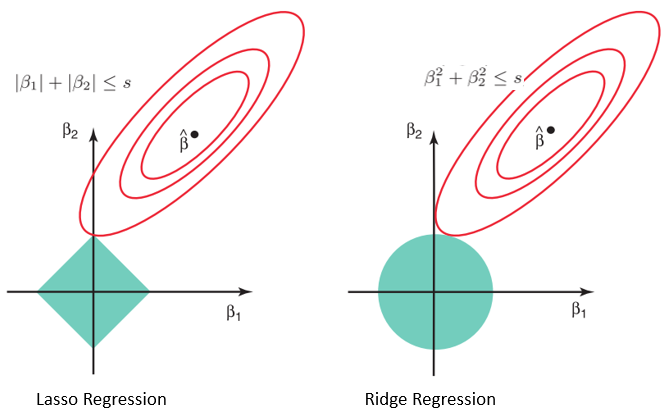
\includegraphics[width=1\linewidth]{fig/geo.png}
	\caption{Geometrijski prikaz $\ell^1$ in $\ell^2$ norme pri LASSO in Ridge regresiji v 2D prostoru parametrov modela.}
	\label{fig:vqvae}
\end{figure}

Na zgornji sliki je primerjava kaznovanja med LASSO in Ridge regresijo. Če enačbo za izračun paramterov v Lagrangeovi obliki zapišemo še za Ridge regresijo, takoj opazimo, da sta si problema na prvi pogled zelo podobna, vendar je razlika velika.

\begin{equation}
	\hat{\beta} =  \underset{\hat{\beta}}{\operatorname{argmin}} \{ ||y - X\beta||_2^2 + \lambda ||\beta||_2 \}
	\label{eqn5} 
\end{equation}

Kot je pokazano v enačbi \eqref{eqn5} pri Ridge regresiji prametre kaznujemo z $\ell^2$ normo. Če meje prikažemo v 2D prostoru parametrov modela, lahko vidimo, da je $\ell^2$ meja pri Ridge regresiji enaka $\beta_1^2 +\beta_2^2 \leq s$ in pri LASSO $|\beta_1| + |\beta_2| \leq s$, pri tem je $s$ stopnja kaznovanja. 

Opazimo, da bo površina, ki jo tvori $\beta_1^2 +\beta_2^2 \leq s$ meja Ridge regresije enaka krogu (v n-dimenzionalnemu prostoru n-krogla) in v primeru LASSO regresije ($|\beta_1| + |\beta_2| \leq s$) kvadrat, ki je rotiran tako, da oglišča ležijo na oseh (v večdimenzionalnem prostoru navzkrižni politop z oglišči na oseh). Ta detajl pokaže, kako LASSO določene parametre nastavi na natanko 0, medtem ko Ridge regresija ne, saj bo kontura parametrov zadela rob meje ravno v oglišču kvadrata (politopa), kar bo povzročilo, da bodo določeni parametri enaki točno 0, medtem ko bodo ostali zavzeli neko vrednost na osi.

\section*{Vrednost $\lambda$ in $t$}

Vrednost $\lambda$ v enačbi \eqref{eqn4} in $t$ v enačbi \eqref{eqn1} direktno nastavljata nivo krčenja (ang. shrinkage), njuno vrednost nastavimo glede na podatke. Tibshirani je v originalnem članu opisal več metod, kako se lahko lotimo nastavitve parametra, največkrat pa ga nastavimo z nazkrižnim preverjanjem. Tibshirani opiše 3 metode:

\begin{itemize}
	\item navzkrižno preverjanje,
	\item generalizirano navzkrižno preverjanje in
	\item analitična nepristranska cenilka tveganja.
\end{itemize}

Največkrat se uporabi kar k-kratno navzkrižno preverjanje, saj ne predpostavlja poznane porazdelitve $X$. S to metodo preverimo različne vrednosti parametrov in najoptimalnejšo določimo glede na rezultate, ki jih model dosega. 

Drugo metodo lahko pridobimo iz linearne aproksimacije za LASSO oceno parametrov modela, tretjo pa z Steinovo nepristransko cenilko tveganja. 

\section{Sample in gene LASSO}

Varianti \emph{sample} in \emph{gene} LASSO se od originalna ne razlikujeta veliko. Še vedno gre za navadno LASSO regresijo, vendar model nekoliko prilagodimo podatkom genske ekspresije.

Meritve genske ekspresije je v zadnjih letih postala popularna in dostopna metoda za raziskovanje bioloških sistemov. V zadnjem desetletju smo bili lahko priča hitremu razvoju metod kot so visoko zmogljivo sekvenciranje (ang. high throughput sequencing) tudi na področju RNA sekvenciranja. Razvite so bile metode kot so RNA sekvenciranje posameznih celic (single-cell RNA-seq) in druge.

Tovrstne metode nam omogočijo, da raziskujemo organizme in posamezna tkiva v zelo visoki resoluciji celo na nivoju posameznih celic. Kljub hitremu razvoju, tovrstne metode še vedno ostajajo drage, sploh ko želimo pridobiti podatke na nivoju celotnega  genoma. S pomočjo analize glavnih komponent so raziskovalci ugotovili, da približno 1000 genov povzame okoli 80 \% variabilnosti vseh genov. To skupino genov so tudi našli in s tem se je začel tudi Library of Integrated Network-Based Cellular Signatures (LINCS) program, ki je pokazal, da lahko s pomočjo 978 mejnih (and. landmark) genov dovolj dobro imputiramo izražanje tisočih ostalih genov. S takšno redukcijo meritev pade cena poskusa na 5 \$ na vzorec. 

\section*{Gene LASSO}

\emph{GeneLASSO} je metoda, ki se veliko uporablja za imputacijo neizmerjenih genov znotraj meritev genske ekspresije. Gre za to, da naučimo nov LASSO model za vsak gen posebej. Tako dobimo $m$ modelov za $m$ genov, ki jih želimo imputirati. Za to seveda potrebujemo celotna podatkovja, torej meritve vseh genov, ki jih želimo uporabiti za imputacijo (torej genov, ki jih bomo izmerili) in vseh genov, ki jih želimo imputirati. 

Ko so modeli naučeni, lahko vsak gen imputiramo z modelom, ki mu pripada. Iz napisanega lahko sklepamo, da bodo te modeli zajeli predvsem variabilnost in odvisnosti, ki se nahajajo med posameznimi geni, ne pa teh, ki se nahajajo med posameznimi vzorci. Za tovrstno imputacijo pa potrebujemo pristop, ki ga zajema \emph{sample LASSO}.

\section*{Sample LASSO}

\emph{Sample LASSO} pa na regresijski problem pogleda ravno obratno, namesto, da izračunamo koeficiente za posamezne gene, v tem primeru izračunamo koeficiente za posamezni vzorec, pri tem pa za treniranje uporabimo vzorec, ki ga želimo imputirati. Gre za to, da prilagodimo najboljši model z uteženo linearno kombinacijo vseh vzorcev, pri tem pa uporabimo samo izmerjene gene (odzivna spremenljivka so izmerjeni geni vzorca, ki ga želimo imputirati, odvisne spremenljivke pa so posamezni vzorci, pri tem pa uporabimo samo gene, ki so izmerjeni). Pričakujemo, da bo LASSO avtomatsko pripisal večjo težo vzorcem, ki so si med sabo podobni in nastavil na nič tiste, ki se zelo razlikujejo od vzorca, ki ga imputiramo.

Ker smo izračunali koeficiente za posamezne vzorce, lahko za imputacijo enostavno utežimo polno izmerjene vzorce, ki jih imamo na voljo in s tem pridobimo vrednosti, ki jih neizmerjeni geni zavzemajo. S ker to naredimo za vzorce, ki imajo merjene vse gene lahko izračunamo tudi mero napake.

\section{Preizkus metod}

Da preizkusim opisano metodo, sem metodi v omejenem obsegu uporabil na podatkih, ki so prosto dostopni na tem naslovu. Gre za zbirko podatkov, ki je bila originalno uporabljena za ta članek. 

\section*{Podatki}

Podatki so javno dostopni na naslovu: \url{https://zenodo.org/record/3971092#.YqnAbHbP2Uk}. Za preizkus sem uporabil podatke iz RNA mikromrež in imputiral RNA mikromreže. 

Predvsem pogledam scenarij, ko bi za imputacijo uporabili starejše \emph{Affymetrix Human Genome U133A Array} (GPL96) mikromreže in imputirali gene, ki jih trenutno lahko merimo samo z novejšimi, genomskimi \emph{Affymetrix Human Genome U133 Plus 2.0 Array} (t.j. GPL570). Na ta način pridobimo podatke označene kot GPL96-570.

Podatki vsebujejo 11678 genov, ki so izmerjeni v obeh mikromrežah, novejše pa imajo še dodatnih 5277 genov, za katere nimamo informacij pri vseh poskusih izvedenih s pomočjo starejših mikromrež. Na voljo je 108 205 vzorcev, ki so bili pridobljeni iz NCBI GEO kot surove CEL datoteke, ki so jim odšteli ozadje, transformirali kvantile, in povzeli s pomočjo fRMA na podlagi po meri narejene kumulativne porazdelitvene funkcije.

\section*{Analiza}

Vsa koda, ki sem jo uporabil se nahaja na tem naslovu: \url{https://github.com/maksobelser/gene-sample_lasso}. 

\end{document}

